\section{Systeme analysieren}
Diese Registerkarte dient zum Berechnen verschiedener Normen. (Abb.9)


\begin{figure}[htb]
\noindent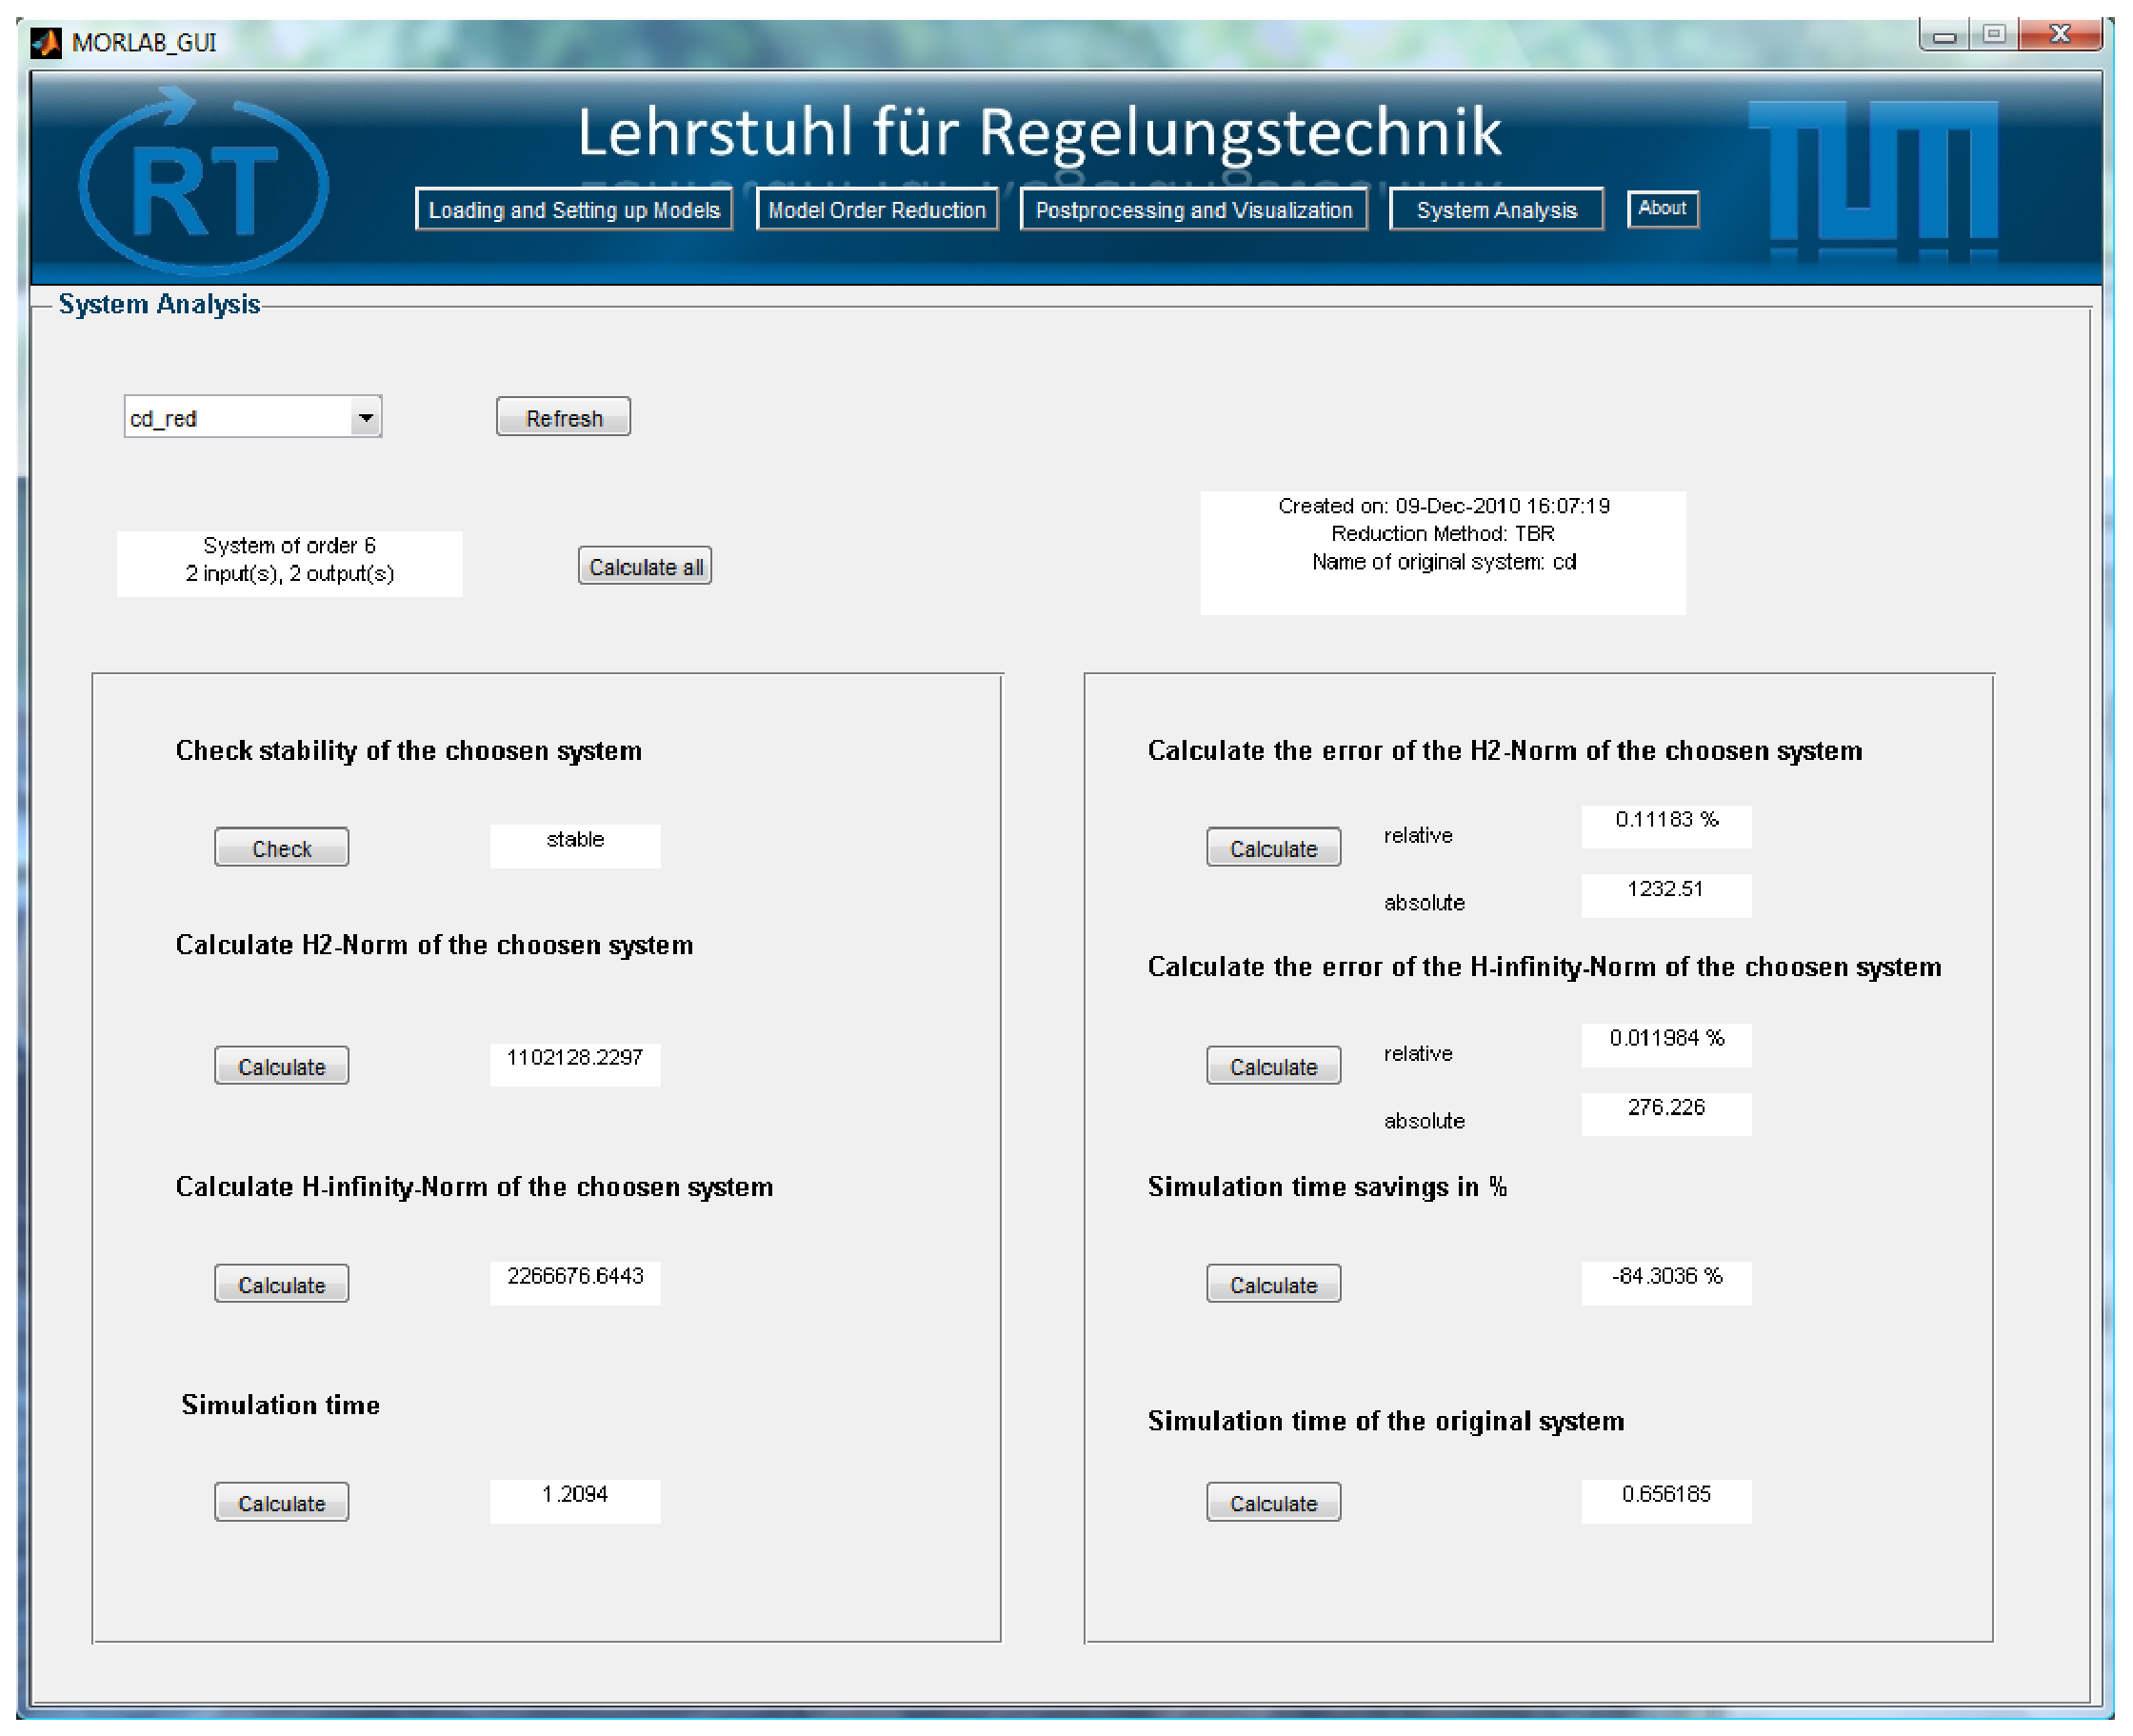
\includegraphics[width=\linewidth,height=\textheight,keepaspectratio]{Abbildungen/tab_analysis}
\caption{Tab Analysis}
\end{figure}

\subsection{System ausw�hlen}
Die Auswahl eines Systems erfolgt wie in den anderen Registerkarten. 
Es gibt zwei Textfelder, in denen Informationen zum ausgew�hlten System angezeigt werden. Im linken erscheinen allgemeine Informationen, wie beispielsweise die Ordnug des Systems, im rechten werden nur Informationen �ber die Reduktion des Systems angezeigt, falls es sich um ein reduziertes System handelt.

\subsection{Analysem�glichkeiten f�r alle Systeme}
Es k�nnen $\mathcal{H}_\infty$- und $\mathcal{H}_2$-Norm berechnet werden, au�erdem die Stabilit�t und eine exemplarische Simulationszeit bestimmt werden. Die exemplarische Simulationszeit ist die Zeit, die der Algorithmus ben�tigt um Pole und Residuen, und damit zu 1000 Zeitpunkten eine Systemantwort zu berechnen.

\subsection{Analysem�glichkeiten f�r reduzierte Systeme}
Bei einem reduzierten System k�nnen au�erdem relativer und absoluter Fehler von $\mathcal{H}_\infty$- und $\mathcal{H}_2$-Norm, die Einsparung in der Simulationszeit und die Simulationszeit des Originalsystems berechnet werden (vorausgesetzt, dieses liegt ebenfalls im Workspace). Da die Fehlersysteme eine h�here Ordnung, als die Orginalsysteme besitzen ist mit einem erh�hten Zeitaufwand zu rechnen.

Mit 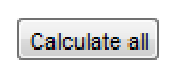
\includegraphics[height=12pt,keepaspectratio]{Abbildungen/pb_calcall} werden alle Felder berechnet. 